\documentclass[aspectratio=169]{beamer} 

\usepackage[utf8]{inputenc}
\usepackage[T1]{fontenc}
\usepackage[bosnian]{babel} 
\usepackage{tikz}
\usepackage{bm} 
\usepackage{caption}
\usepackage{subcaption}
\usepackage{float}
\usepackage{transparent}

% Workaround so I can keep theme files in a subfolder,
% as per https://tex.stackexchange.com/a/284157/181620
\makeatletter
  \def\beamer@calltheme#1#2#3{%
    \def\beamer@themelist{#2}
    \@for\beamer@themename:=\beamer@themelist\do
    {\input{theme/source/_build/#3\beamer@themename.sty}}}
\usetheme{metropolis}

\usepackage{xcolor}
\usepackage[outline]{contour}
\contourlength{2pt}
\contournumber{7}

\captionsetup{labelformat=empty}

% Add framesubtitle to template
\setbeamercolor{framesubtitle}{fg=mDarkTeal}
\addtobeamertemplate{frametitle}{}{%
  \ifx
    \large
    \insertframesubtitle\@empty
  \else%
    \usebeamerfont{framesubtitle}%
    \usebeamercolor[fg]{framesubtitle}%
    \vskip10pt
    \large
    \insertframesubtitle%
  \fi%
}

\graphicspath{{img/}{../_build/img/}}

\title {
  Jednodimenzionalne i višedimenzionalne normalne raspodjele, zakoni velikih
  brojeva i centralni granični teorem
}
\author{Haris Gušić}

\begin{document}

  \begin{frame}
    \maketitle
  \end{frame}

{

	\setbeamertemplate{background} {
		\begin{tikzpicture}
			\node[opacity=0.06, inner sep=0] {
				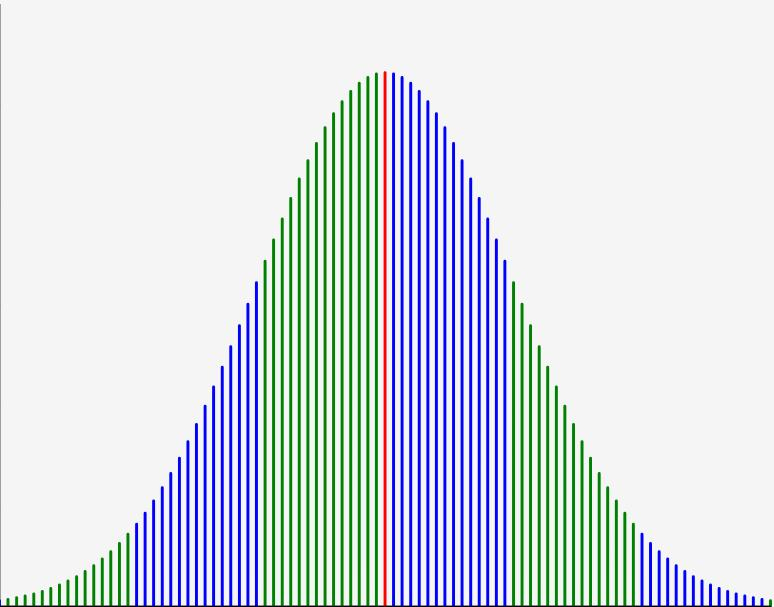
\includegraphics[trim=0cm 0cm 0cm -4cm, width=\paperwidth, height=1\paperheight]
				{gauss}
			};
		\end{tikzpicture}
	}

  \begin{frame}{Normalna raspodjela}{Jedna slučajna varijabla}
    \begin{itemize}
      \item $X \sim \mathcal{N}(\mu,\sigma^2)$
      \item PDF
        $$p_X(x) = \frac{1}{\sqrt{2\pi\sigma^2}} e^{-\frac{(x-\mu)^2}{2\sigma^2}}$$
      \item Očekivanje: $\mu$, Varijansa: $\sigma^2$
      \item Često se susreće u praksi
      \item Povezana sa centralnim graničnim teoremom
    \end{itemize}
  \end{frame}

}

  \begin{frame}{Normalna raspodjela}{Jedna slučajna varijabla}
    \vspace{.3cm}
    \begin{itemize} \item Izgled PDF \end{itemize}
    \vspace{.3cm}
    \begin{figure}[ht]
      \begin{minipage}[b]{0.45\linewidth}
        \centering
        \includegraphics[height=4cm]{gauss_uni_std}
        \caption{$\mu=0, \sigma=1$}
      \end{minipage}
      \hspace{0.5cm}
      \begin{minipage}[b]{0.45\linewidth}
        \centering
        \includegraphics[height=4cm]{gauss_uni_deltavar}
        \caption{$\mu=-2, \sigma=2$}
      \end{minipage}
     \caption
     \hfill
    \end{figure}
  \end{frame}
  
  \begin{frame}{Normalna raspodjela}{Jedna slučajna varijabla}
    \begin{itemize}
      \item CDF
        \begin{itemize}
          \item[-] Nema zatvorenog oblika
          \item[-] Standardna normalna raspodjela:
            $$P_X(x) = \Phi(x) = \frac{1}{\sqrt{2\pi}} \int_{-\infty}^{x}
            e^{-\frac{x^2}{2}} \ \mathrm dx$$
          \item[-] Sa očekivanjem $\mu$ i varijansom $\sigma^2$:
            $$P_X(x) = \Phi\left(\frac{x-\mu}{\sigma}\right)$$
        \end{itemize}
    \end{itemize}
  \end{frame}

{

	\setbeamertemplate{background} {
		\begin{tikzpicture}
			\node[opacity=0.06, inner sep=0] {
				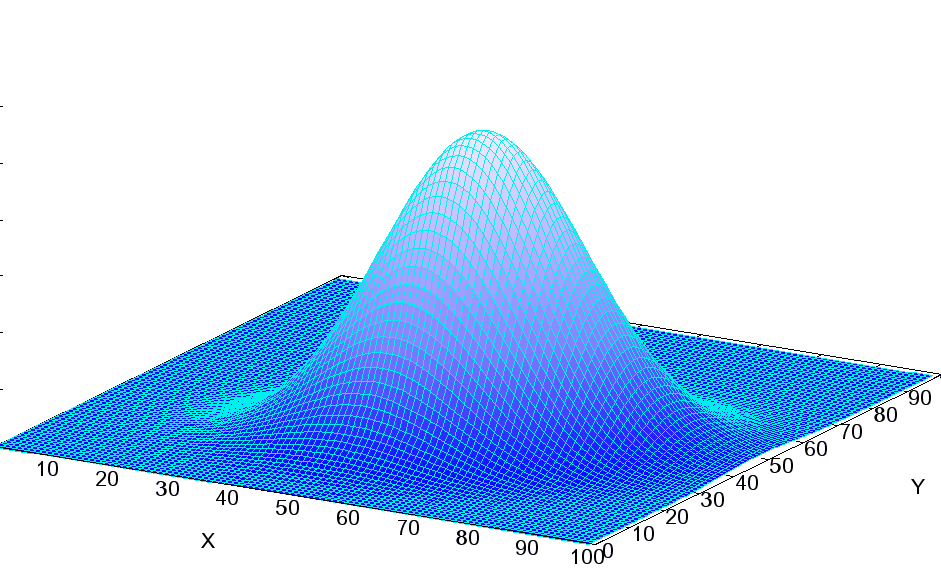
\includegraphics[trim=0cm 0cm 0cm 1cm, width=\paperwidth]
				{gauss-multi.png}
			};
		\end{tikzpicture}
	}

  \begin{frame}{Normalna raspodjela}{Multivarijabilna}
    \begin{itemize}
      \item Slučajni vektor
        $$\bm X = [ X_1\ X_2\ \cdots\ X_k]^\mathrm T$$
      \item $\bm X \sim \mathcal{N}(\bm\mu, \bm C_{\bm X\bm X})$
      \item PDF
        $$p_{\bm X}(\bm x) 
        = \frac{1}{\sqrt{(2\pi)^k \det \bm C_{\bm X \bm X}}} e^{ -\frac{1}{2}(\bm x -
          \bm\mu_{\bm X})^\text T \bm C_{\bm X \bm X}^{-1} (\bm x - \bm\mu_{\bm
        X})}$$
      \item Očekivanje: $\bm\mu_{\bm X}$, kovarijantna matrica $\bm C_{\bm X\bm
        X}$

    \end{itemize}
  \end{frame}
}

  \begin{frame}{Multivarijabilna normalna raspodjela}{Analogije}
    $$p_X(x) = \frac{1}{\sqrt{2\pi\sigma_X^2}} e^{-\frac{(x-\mu_X)^2}{2\sigma_X^2}}$$
    $$p_{\bm X}(\bm x) 
    = \frac{1}{\sqrt{(2\pi)^k \det \bm C_{\bm X \bm X}}} e^{ -\frac{1}{2}(\bm x -
      \bm\mu_{\bm X})^\text T \bm C_{\bm X \bm X}^{-1} (\bm x - \bm\mu_{\bm
      X})}$$
    \vspace{15pt}
    \hrule
    %
    $$\mu_X \longleftrightarrow \bm\mu_{\bm X}$$
    %
    $$\sigma_X^2 \longleftrightarrow \bm C_{\bm X\bm X}$$
    %
    $$ \frac{(x-\mu_X)^2}{\sigma_X^2} \longleftrightarrow
      (\bm x-\bm\mu_{\bm X})^\text T \bm C_{\bm X \bm X}^{-1}
      (\bm x - \bm\mu_{\bm X})$$
    $$2\pi \longleftrightarrow (2\pi)^k$$
  \end{frame}

  \begin{frame}{Multivarijabilna normalna raspodjela}{Slučaj dvije varijable}
    $$ \bm\mu_{\bm X} = [\mu_1\ \mu_2]^\mathrm T,\ 
      \bm C_{\bm X\bm X} = \left[\begin{array}{cc}
        \sigma_1^2 & \rho\sigma_1\sigma_2 \\  \rho\sigma_1\sigma_2 & \sigma_2^2
        \end{array}\right] $$
    \begin{itemize}
      \item Marginalne raspodjele:
        $$X_1 \sim \mathcal{N}(\mu_1, \sigma_1^2)$$
        $$X_2 \sim \mathcal{N}(\mu_2, \sigma_2^2)$$
    \end{itemize}
  \end{frame}

  \begin{frame}{Multivarijabilna normalna raspodjela}{Demonstracija (Jupyter)}
    \begin{figure}[ht]
      \begin{minipage}[b]{0.45\linewidth}
        \centering
        \includegraphics[width=0.6\textwidth]{gauss_multi_std}
      \end{minipage}
      \begin{minipage}[b]{0.45\linewidth}
        \centering
        \includegraphics[width=0.6\textwidth]{gauss_multi_corr+}
      \end{minipage}
    \end{figure}
  \end{frame}
  
  \begin{frame}{Zakon velikih brojeva}{Primjer novčića}
    \begin{itemize}
      \item Dvije mogućnosti: "Glava" (0), "Pismo" (1)
      \item Eksperiment: bacanje novčića $n$ puta
      \item Primjer ishoda eksperimenta: \textit{PGGPGPGGGPP (10010100011)}
      \item Zadatak: \textbf{Prebrojati koliko puta se pojavilo pismo u $n$
        bacanja} ($K_n$).
    \end{itemize}
  \end{frame}

  \begin{frame}{Primjer novčića}
    \begin{itemize}
      \item Novčić je nepravedan, $p(1)=p,\ p(0)=q$
      \item $K_n$ ima \textit{binomnu} raspodjelu
        $$p_{K_n}(k) = \binom{n}{k}p^kq^{n-k},\ \mu_{K_n}=np$$
      \item Za $p=q=0.5$, $n=8$:
      \begin{figure}
        \centering
        \includegraphics[width=0.4\textwidth]{clt_binom_8}
      \end{figure}
    \end{itemize}
  \end{frame}
  
  \begin{frame}{Primjer novčića}
    \begin{itemize}
      \item Relativna frekvencija $\frac{K_n}{n}$
      \item Slučajna sekvenca (proces) $\{X_i\}$, $X_i \in \{0,1\}$
      \item Slučajna sekvenca $\{S_n\}$ \textit{srednjih vrijednosti uzoraka
        (sample mean)}
        $$S_1=X_1,\ S_2=\frac{X_1+X_2}{2},\ S_3=\frac{X_1+X_2+X_3}{3},...$$
        $$\boxed{\frac{K_n}{n} = S_n = \frac{1}{n} \sum_{i=1}^n X_i}$$
      \item \textbf{Primjer:} \textit{01110}, $S_5=(0+1+1+1+0)/5=3/5$
    \end{itemize}
  \end{frame}
  
  \begin{frame}{Zakoni velikih brojeva}
    \begin{itemize}
      \item Za dovoljno veliko $n$:
        \begin{equation*}
          S_n \approx \mu_{X_n} = p
        \end{equation*}
      \item Koliko smo sigurni u ovu procjenu? (CLT) %TODO move
      \item $X_n$ može biti opća sekvenca
    \end{itemize}
  \end{frame}

  \begin{frame}{Zakoni velikih brojeva}{Slabi zakon}
    \begin{itemize}
      \item Uslov: sekvenca $X_n$ nezavisna, $\mu_{X_n}=\mu_X$, varijanse
        $\sigma_n$ ograničene kad $n\to\infty$
      $$\lim_{n\to\infty} P \left(|S_n - \mu_X| < \varepsilon\right) = 1$$
      \item "Svaka realizacija vjerovatno dovoljno dobro teži ka $\mu_X$"
      \item Prevedeno: velik broj eksperimenata $\implies$ dobra procjena $\mu$
      \item Specijalan slučaj: IID proces
    \end{itemize}
  \end{frame}

  \begin{frame}{Zakoni velikih brojeva}{Jaki zakon}
    \begin{itemize}
      \item Vrijedi za IID sekvence sa konačnom varijansom
      $$\lim_{n\to\infty} S_n = \mu_X \text{ skoro sigurno}$$
      \item "Praktično je sigurno da će svaka realizacija konvergirati"
    \end{itemize}
  \end{frame}
  
  \begin{frame}{Zakoni velikih brojeva}{Demonstacija (Jupyter)}
    \vspace{10pt}
    \begin{figure}
      \begin{minipage}[b]{0.27\linewidth}
        \centering
        \includegraphics[width=\textwidth]{lln_demo_1}
      \end{minipage}
      \begin{minipage}[b]{0.27\linewidth}
        \centering
        \includegraphics[width=\textwidth]{lln_demo_2}
      \end{minipage}
      \\
      \begin{minipage}[b]{0.27\linewidth}
        \centering
        \includegraphics[width=\textwidth]{lln_demo_3}
      \end{minipage}
      \begin{minipage}[b]{0.27\linewidth}
        \centering
        \includegraphics[width=\textwidth]{lln_demo_4}
      \end{minipage}
    \end{figure}
  \end{frame}
  
  \begin{frame}{Zakoni velikih brojeva}{Praktična primjena + demonstracija}
    \begin{itemize}
      \item Niz eksperimenata (mjerenja)
      \item Veličina se ne mijenja u vremenu
      \item Događaj "mjerenje je u opsegu $[a,b]$"
      \item \textbf{Histogram aproksimira PDF}
    \end{itemize}
    \begin{figure}
      \begin{minipage}[b]{0.27\linewidth}
        \centering
        \includegraphics[height=2.6cm]{lln_hist_1}
      \end{minipage}
      \hspace{0.5cm}
      \begin{minipage}[b]{0.27\linewidth}
        \centering
        \includegraphics[height=2.6cm]{lln_hist_2}
      \end{minipage}
      \hspace{0.5cm}
      \begin{minipage}[b]{0.27\linewidth}
        \centering
        \includegraphics[height=2.6cm]{lln_hist_3}
      \end{minipage}
    \end{figure}
  \end{frame}

{

  % Dice image is part of epsdice package
	\setbeamertemplate{background} {
		\begin{tikzpicture}
			\node[opacity=0.04, inner sep=0] {
				\includegraphics[trim=0cm 0cm -2cm -2cm, height=\paperheight]
				{dice}
			};
		\end{tikzpicture}
	}

  \begin{frame}{Centralni granični teorem}{Suma nezavisnih slučajnih varijabli}
    \begin{itemize}
      \item Par (pravednih) igraćih kocki ($1,2,3,4,5,6$)
      \item Slučajne varijable $X_1$, $X_2$, $S=X_1+X_2$
      \item Kocke su nezavisne
      \item \textbf{Kolika je vjerovatnoća da je suma = 4?}
    \end{itemize}
  \end{frame}

}
  
  \begin{frame}{Suma nezavisnih slučajnih varijabli}
    $$p_S(4) = p_{X_1}(1)p_{X_2}(4-1) + p_{X_1}(2)p_{X_2}(4-2) +
      p_{X_1}(3)p_{X_2}(4-3)$$
    \begin{itemize}
      \item PMF:
        $$p_{S}(n) = \sum_{k=-\infty}^{\infty} p_{X_1}(k) p_{X_1}(n-k)$$
      \item Opći slučaj (nezavisne varijable):
        $$p_S(s) = p_{X_1} * p_{X_2} * \cdots * p_{X_n} (s)$$
    \end{itemize}
  \end{frame}

  \begin{frame}{Suma nezavisnih slučajnih varijabli}{Ponovo novčić}
    \begin{itemize}
      \item $K$ broj ishoda "Pismo" u $n$ bacanja.
        $$K = \sum_{i=1}^{n} X_i$$
      \item PMF:
        $$p_K(k) = \underbrace{p_X * p_X * \cdots * p_X (k)}_{n\text{ puta}}$$
    \end{itemize}
  \end{frame}

  \begin{frame}{Suma nezavisnih slučajnih varijabli}{Demonstracija (Jupyter)}
    \begin{figure}
      \begin{minipage}[b]{0.27\linewidth}
        \centering
        \includegraphics[width=\textwidth]{clt_binom_1}
      \end{minipage}
      \begin{minipage}[b]{0.27\linewidth}
        \centering
        \includegraphics[width=\textwidth]{clt_binom_2}
      \end{minipage}
      \begin{minipage}[b]{0.27\linewidth}
        \centering
        \includegraphics[width=\textwidth]{clt_binom_3}
      \end{minipage}
      \\
      \begin{minipage}[b]{0.27\linewidth}
        \centering
        \includegraphics[width=\textwidth]{clt_binom_8}
      \end{minipage}
      \begin{minipage}[b]{0.27\linewidth}
        \centering
        \includegraphics[width=\textwidth]{clt_binom_50}
      \end{minipage}
    \end{figure}
  \end{frame}

  \begin{frame}{Suma nezavisnih slučajnih varijabli}{Zaključci}
    \begin{itemize}
      \item Vrijednosti u sredini su vjerovatnije
      \item Vrijednosti na rubovima su malo vjerovatne
      \item Opseg vrijednosti se širi
      \item Raspodjela aproksimira normalnu (De Moivre-Laplace)
    \end{itemize}
  \end{frame}
  
  \begin{frame}{Centralni granični teorem}
    \begin{itemize}
      \item \textbf{Suma velikog broja IID slučajnih varijabli $X_i$ je
        približno normalno raspodijeljena!}
      \item Normalizacija:
        $$S_n = \frac{1}{\sqrt{n}}\sum_{i=1}^{n} \frac{X_i-\mu}{\sigma}$$
      \item Formalno
        $$\lim_{n\to\infty} P_{S_n}(s) = \mathcal{N}(0,1)$$
      \item Dokaz (koga zanima) je dat u radu
    \end{itemize}
  \end{frame}

  \begin{frame}{Centralni granični teorem}{Osobina konvolucije, demonstracija
    (Jupyter)}
    \begin{figure}
      \begin{minipage}[b]{0.27\linewidth}
        \centering
        \includegraphics[height=3cm]{clt_conv_noise}
      \end{minipage}
      \hspace{0.5cm}
      \begin{minipage}[b]{0.27\linewidth}
        \centering
        \includegraphics[height=3cm]{clt_conv_noise_1}
      \end{minipage}
      \hspace{0.5cm}
      \begin{minipage}[b]{0.27\linewidth}
        \centering
        \includegraphics[height=3cm]{clt_conv_noise_2}
      \end{minipage}
    \end{figure}
  \end{frame}

  \begin{frame}{Centralni granični teorem}{Veza sa LLN}
    \begin{itemize}
      \item Sekvenca srednjih vrijednosti uzoraka aproksimira normalnu raspodjelu.
      \item Raspodjela se sužava sa povećanjem $n$
        \begin{figure}
          \centering
          \includegraphics[width=0.4\textwidth]{clt_degen}
        \end{figure}
      \item Za $n\to\infty$, $p_{S_n}(x) \approx \delta(x-\mu)$
    \end{itemize}
  \end{frame}

  \begin{frame}{Centralni granični teorem}{Praktične primjene}
    \begin{itemize}
      \item Objašnjava zašto se normalna raspodjela susreće toliko često
      \item Fenomeni su često nezavisni ili slabo korelirani
      \item Optičko vlakno
      \item Generisanje slučajnih brojeva
      \item Moving average filteri
    \end{itemize}
  \end{frame}

  \begin{frame}
    \textbf{\Huge Hvala na pažnji}
  \end{frame}
  
\end{document}
